
\section{Outros Métodos}

\subsection{Método pela Resolução}

\begin{frame}[t]
\vskip 3cm
\begin{center}
{\Huge Método pela Resolução}
\end{center}

\end{frame}


\begin{frame}{Definição:}

A resolução é um método de dedução, que também define uma estrutura para 
representação e dedução de conhecimento. Não temos axiomas, apenas uma 
regra de inferência. Utilizamos na prova de argumentos a partir do 
conhecimento representado no sistema. A prova é feita aplicando a regra 
de resolução sobre um conjunto de cláusulas.

\vspace{0.7cm}

De forma dual, a resolução se aplica a fórmulas que são
 conjunções de disjunções de literais,representadas na forma 
 de conjunto de cláusulas. A linguagem de programação ProLoG, 
 é um exemplo de utilização desse método.


\end{frame}

\begin{frame}{Notação:}

Representação na forma de conjunto de cláusulas:\\

Exemplo: $$H = (p \vee \sim q \vee r) \wedge (p \vee \sim q) \wedge  (p \vee p)$$  

A representação na forma de {\bf conjunto de cláusulas} fica:\\
         
$$H = \{\{p,\sim q,r\},\{p,\sim q\},\{p\}\}$$

Onde as vírgulas internas representam as disjunções ($\vee$) e as externas as conjunções ($\wedge$).

OBS: Quanto à representação do último termo do conjunto, note que:\\
		 $$(p \vee p) = \{p,p\} = \{p\}$$
\end{frame}




\begin{frame}{Cláusulas}
Definição: na Lógica Proposicional uma cláusula é uma disjunção de literais.
\vspace{0.5cm}
Exemplo: Utilizando o conjunto de cláusulas do exemplo anterior:
\\
\begin{table}
\centering
\begin{tabular}{l}
\hline
\hline
$C_1 = \{p, \sim q, r\}$\\ \hline
$C_2 = \{p,\sim q\}$\\  \hline
$C_3 = \{p\}$\\
\hline
\hline
\end{tabular}
\end{table}
              
Assim, H possui 3 cláusulas: $C_1,C_2$ e $C_3$

\end{frame}

\begin{frame}{Literais Complementares}
Definição: para serem complementares, um literal deverá ser a negação do outro.
\begin{table}
\centering
\begin{tabular}{r|r}
\hline
\hline
$p$&$\sim p$\\
\hline
$q$&$\sim q$\\
\hline
\hline
\end{tabular}
\end{table}
\end{frame}
%%%%%%%%%%%%%%%%%%%%%%%%%%%%%%%%%%%%%%%%%%
\begin{frame}
\frametitle{Resolvente de Duas Cláusulas}

Definição: sejam duas cláusulas:
$$C_1 = \{a_1,...,a_n\} $$ 
$$C_2 = \{b_1,...,b_n\}$$

\begin{itemize}
\item Considere que ambas possuem literais complementares.

\item Agora,  supondo que há um literal $\lambda$
em $C_1$ e  seu complemento $\sim \lambda$ em $C_2$.

\item O resolvente $Res(C_1,C_2)$ é definido por:
\begin{equation}
Res(C_1,C_2) = (C_1 - \lambda) \cup (C_2 - \sim \lambda)
\label{equacao_resolvente}
\end{equation}
\item Se $Res(C_1,C_2) = \{\}$, dizemos que temos um \textit{resolvente vazio} ou \textit{trivial}

\end{itemize}
\end{frame}

\begin{frame}{Exemplos:}

\begin{itemize}
%%% ESPACAMENTO ENTRE ITEnS
\itemsep 0.7cm

\item $C_1 = \{p,\sim q, r\}$ e $C_2 = \{ \sim p, r\}$ O resolvente de $C_1$ e $C_2$ é dado por:\\
\begin{center}
$Res(C_1,C_2) = \{ \sim q, r \}$
\end{center}

O resolvente de $C_1$ e $C_2$ também é uma cláusula e $\lambda = p$.\\

\item $D_1 = \{p\}$ e $D_2 = \{ \sim p\}$ O resolvente de $D_1$ e $D_2$ é dado por $$Res(D_1,D_2) = \{ \}$$

Neste caso, o resolvente das duas cláusulas é a cláusula vazia  e $\lambda = p$.
\end{itemize}
\end{frame}
%%%%%%%%%%%%%%%%%%%%%%%%%%%%%%%%%%%%%%%%%%%%%%%%%5

\begin{frame}
%%% ESPACAMENTO ENTRE ITEnS


\begin{itemize}
\itemsep 0.7cm

\item $E_1 = \{p, \sim q\}$ e $E_2 = \{ \sim p, q\}$

$$Res(E_1,E_2) = \{ \sim q, q\}$$

Agora, a resolução não elimina todos os literais das cláusulas mesmo eles sendo complementares.
\end{itemize}

\end{frame}

\begin{frame}{Regra de Resolução}

\begin{itemize}
\itemsep 0.7cm
\item O mecanismo de inferência da resolução utiliza apenas uma regra que é semelhante à Modus Ponens, porém mais adequada às implementações em computadores.

\item A regra de resolução é definida  a partir
de duas cláusulas quaisquer
$$C_1 = \{a_1,...,a_n \}$$ 
$$C_2 = \{ b1,...,bn\}$$
tal que a regra de resolução aplicada a $C_1$ e $C_2$ é definida pelo procedimento a seguir:
\end{itemize}
\end{frame}

\begin{frame}{Expansão por Resolução}

\begin{itemize}
\itemsep 0.7cm

\item Onde $C_1$ e $C_2$ com seus termo $\lambda $ em $C_1$ e $\sim \lambda $ em $C_2$, aplique  $Res(C_1,C_2)$ definida na equação \ref{equacao_resolvente}

\item Essencialmente é a aplicação do passo anterior sucessivas vezes, até encontrar a cláusula vazia. Se esta for encontrada, há uma contradição.

\item A regra de resolução é aplicada repetidamente, até que se consiga obter a cláusula vazia. Essa aplicação repetida da regra de resolução determina uma \textit{expansão por resolução}.

\end{itemize}

\end{frame}

\begin{frame}{Exemplos:}
Considere o conjunto de cláusulas:

$\{\{ \sim p, q, r\},\{p, r\},\{p, \sim r\}\}.$

Uma expansão por resolução sobre esse conjunto é:

\begin{table}
\centering
\begin{tabular}{r|l|r}
\hline
\hline
$1.$&$\{ \sim\ p, q, r\}$&$ $\\
\hline
$2.$&$\{p,r\}$&$ $\\
\hline
$3.$&$\{p,\sim r\}$&$ $\\
\hline
$4.$&$ \{q,r\}$&$Res(1,2)$\\
\hline
$5.$&$ \{q,p\}$&$Res(3,4)$\\
\hline
$6.$&$ \{p\}$&$Res(2,3)$\\
\hline
\hline
\end{tabular}
\end{table}

A expansão acima é obtida por três aplicações da regra de resolução. Neste exemplo, não foi possível obter a cláusula vazia.
OBS: A obtenção da cláusula vazia é uma propriedade importante. Quando ocorre, chamamos de \texttt{Expansão por Resolução Fechada}.

\end{frame}

\begin{frame}{Prova por Resolução}

\begin{itemize}
\item Seja $H$ é um teorema lógico por {\bf H}ipótese

\item Não se sabe se é verdade ou falso

\item Supondo que seja teorema lógico, então será  uma tautologia

\item Logo, $\sim H$ deverá ser uma inconsistência


\item Definição: seja $H$ uma fórmula e $\sim H_c$ a forma clausal associada a $\sim H$. Uma prova de $H$ por resolução é uma expansão por resolução fechada sobre $\sim H_c$. Neste caso, $H$ é um teorema do sistema de resolução.

\end{itemize}

%%%%%%%%%%%%%%%%%%%%%%%%%%%%%%%%%%%%%%%%%%%%%%%%%%%%%%%%%%%%%

\end{frame}

\begin{frame}{Exemplo de Prova por Resolução:}
 \textcolor{blue}{Exemplo 1:} 

Considere a fórmula: 

$H=((p_1 \vee p_2 \vee p_3) \wedge (p_1 \rightarrow p_4) \wedge (p_3 \rightarrow p_4)) \rightarrow p_4$

Relembrando tudo:

\begin{itemize}
\item Seja $H=((p_1 \vee p_2 \vee p_3) \wedge (p_1 \rightarrow p_4) \wedge (p_3 \rightarrow p_4)) \rightarrow p_4$

\item Isto é: $((p_1 \vee p_2 \vee p_3) \wedge (p_1 \rightarrow p_4) \wedge (p_3 \rightarrow p_4)) \vdash p_4$

\item ou ainda  $\{(p_1 \vee p_2 \vee p_3) \wedge (p_1 \rightarrow p_4) \wedge (p_3 \rightarrow p_4)\} \vdash p_4$

\item ou ainda  $\{(p_1 \vee p_2 \vee p_3) , (p_1 \rightarrow p_4) , (p_3 \rightarrow p_4)\} \vdash p_4$

\item Nenhuma alteração foi feita, apenas reescrevemos o exercício.

\item Bem como:  $\Phi(\{(p_1 \vee p_2 \vee p_3) , (p_1 \rightarrow p_4) , (p_3 \rightarrow p_4)\} \vdash p_4) \equiv \blacksquare$

\item com rigor: $\Phi(\{(p_1 \vee p_2 \vee p_3) , (p_1 \rightarrow p_4) , (p_3 \rightarrow p_4)\} \rightarrow p_4) \equiv \blacksquare$

\item Ou seja  $\Phi(H) = \blacksquare$

\item Logo, $\Phi(\sim H) = \square$

\end{itemize}
\end{frame}

\begin{frame}

\begin{itemize}
\item \textcolor{blue}{Primeiro passo}: 

determinar uma forma clausal $\sim H_c$ associada a $\sim H$. A fórmula $\sim H_c$ é determinada considerando as equivalências a seguir:

$\scriptstyle \sim H = \sim (((p_1 \vee p_2 \vee p_3) \wedge (p_1 \rightarrow p_4) \wedge (p_2 \rightarrow p_4) \wedge (p_3\rightarrow p_4) \rightarrow p_4$ 
\\
equivale a:
\\
$\scriptstyle \sim (\sim ((p_1 \vee p_2 \vee p_3) \wedge (\sim p_1 \vee p_4) \wedge (\sim p_2 \vee p_4) \wedge (\sim p_3 \vee p_4) \vee p_4$ 
\\
equivale a: 
\\
$\scriptstyle (p_1 \vee p_2 \vee p_3) \wedge (\sim p_1 \vee p_4) \wedge (\sim p_2 \vee p_4) \wedge (\sim p_3 \vee p_4) \wedge \sim p_4 = \sim H_c$

\end{itemize}
\end{frame}

\begin{frame}{Exemplo de Prova por Resolução:}
\begin{itemize}
\item  \textcolor{blue}{Segundo passo:} 
\\
observe que a fórmula $\sim H_{clausulas}$ é uma conjunção de cláusulas e é representada como:
\\
$$\scriptstyle \sim H_c = \{\{p_1, p_2, p_3\},\{\sim p_1, p_4\},\{\sim p_2, p_4\},\{\sim p_3, p_4\},\{\sim p_4\}\}$$
\end{itemize}
\end{frame}


\begin{frame}{Exemplo de Prova por Resolução:}
\begin{itemize}
\item  \textcolor{blue}{Terceiro passo:} 

desenvolver uma expansão por resolução sobre $\sim Hc$.
\begin{table}
\centering
\begin{tabular}{r|l|r}
\hline
\hline
$1.$&$\{p1,p2,p3\}$&$ $\\
\hline
$2.$&$\{\sim p1,p4\}$&$ $\\
\hline
$3.$&$\{\sim p2,p4\}$&$ $\\
\hline
$4.$&$\{\sim p3,p4\}$&$ $\\
\hline
$5.$&$\{\sim p4\}$&$ $\\
\hline
$6.$&$\{p2,p3,p4\}$&$Res(1,2)$\\
\hline
$7.$&$\{p3,p4\}$&$Res(3,6)$\\
\hline
$8.$&$\{p4\}$&$Res(4,7)$\\
\hline
$9.$&$\{  \}$&$Res(5,8)$\\
\hline
\hline
\end{tabular}
\end{table}

A expansão por resolução é fechada, portanto temos uma prova de H.

\end{itemize}
\end{frame}

\begin{frame}
\begin{figure}[!htb]
\centering 
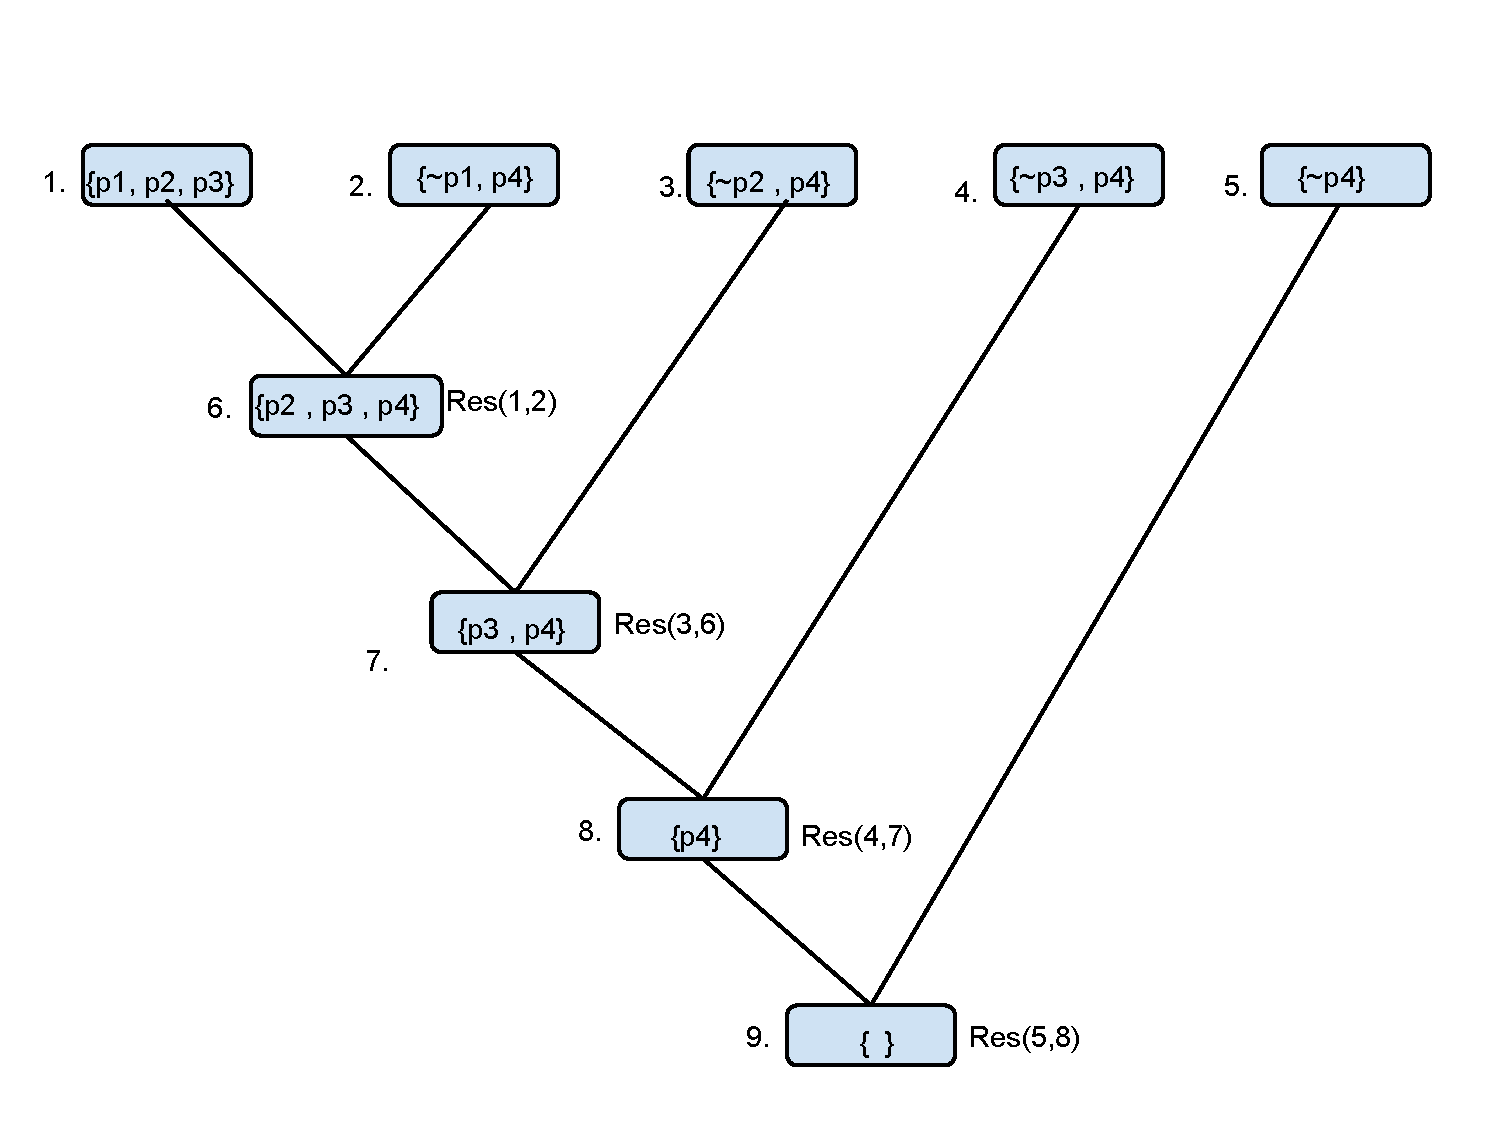
\includegraphics[width=1\textwidth]{arvore_metodo_resolucao.pdf}
\caption{Exemplo de Prova por Resolução}
\label{fig_arvore_resolucao}
\end{figure}

\end{frame}

\begin{frame}{Exemplo de Prova por Resolução:}
 \textcolor{blue}{Exemplo 2:}
 \begin{itemize}
\item Considere as fórmulas
\vspace{0.5cm}

$G=((p1 \vee p2)\wedge(p1\rightarrow p4)\wedge(p2\rightarrow p4)\wedge(p3\rightarrow p4))\rightarrow p3$
\vspace{0.5cm}

\item Considerando as equivalências:
\vspace{0.5cm}

$\sim G=\sim(((p1\vee p2)\wedge(p1\rightarrow p4)\wedge(p2\rightarrow p4)\wedge(p3\rightarrow p4))\rightarrow p3)$
\vspace{0.5cm}

\item equivale a:

$\sim(\sim((p1\vee p2)\wedge(\sim p1\vee p4)\wedge(\sim p2\vee p4)\wedge(\sim p3\vee p4))\vee p3$
\vspace{0.5cm}

\item equivale a:

$(p1\vee p2)\wedge(\sim p1\vee p4)\wedge(\sim p2\vee p4)\wedge(\sim p3\vee p4)\wedge \sim p3=\sim Gc$
\end{itemize}
\end{frame}

\begin{frame}{Exemplo de Prova por Resolução:}
Na notação de conjuntos $\sim Gc$ é:

$\sim Gc = \{\{p1,p2\},\{\sim p1,p4\},\{\sim p2,p4\},\{\sim p3,p4\},\{\sim p3\}\}$

Uma expansão por resolução sobre $\sim Gc$ é dada por:
\\
\begin{table}
\centering
\begin{tabular}{r|l|r}
\hline
\hline
$1.$&$\{p1,p2\}$&$ $\\
\hline
$2.$&$\{\sim p1,p4\}$&$ $\\
\hline
$3.$&$\{\sim p2,p4\}$&$ $\\
\hline
$4.$&$\{\sim p3,p4\}$&$ $\\
\hline
$5.$&$\{\sim p3\}$&$ $\\
\hline
$6.$&$\{p2,p4\}$&$Res(1,2)$\\
\hline
$7.$&$\{p4\}$&$Res(3,6)$\\
\hline
\hline
\end{tabular}
\end{table}

Neste caso a expansão por resolução não é fechada. Portanto, não temos a prova de $G$.
\end{frame}


\begin{frame}{Consequência Lógica por Resolução}
Dada uma fórmula H e um conjunto de hipóteses

$\beta = \{a1,...,an\}$,

então H é uma consequência lógica de $\beta$, por resolução, se existe uma prova de

$(a1 \wedge ... \wedge an) \rightarrow H $

por resolução.
\end{frame}

\begin{frame}{Exemplo de Consequência Lógica por Resolução}

Seja o exemplo:
\begin{enumerate}
\item Guga é determinado.

\item Guga é inteligente.

\item Se Guga é determinado e atleta, ele não é um perdedor.

\item Guga é um atleta se é um amante do tênis.

\item Guga é amante do tênis se é inteligente.
\end{enumerate}

Demonstre que: ``\textit{Guga não é um perdedor}" é uma consequência lógica dos argumentos acima?
\end{frame}

\begin{frame}{Exemplo de Consequência Lógica por Resolução}
\begin{itemize}
\item Demonstra-se a seguir, utilizando resolução, que a consequência lógica ocorre.
\vspace{0.7cm}

\item Conforme foi analisado anteriormente, a representação dos argumentos na Lógica Proposicional é dada por:
\vspace{0.7cm}

$H = (p \wedge q \wedge ((p \wedge r) \rightarrow \sim p1) \wedge (q1 \rightarrow r) \wedge (q \rightarrow q1)) \rightarrow \sim p1$
\end{itemize}
\end{frame}

\begin{frame}{Exemplo de Consequência Lógica por Resolução}
A forma clausal associada a $\sim H$ é obtida pelas equivalências:

$\sim H = \sim((p \wedge q\wedge((p\wedge r)\rightarrow \sim p1)\wedge(q1 \rightarrow r)\wedge (q \rightarrow q1))\rightarrow \sim p1)$

equivale a:

$\sim(\sim(p \wedge q \wedge((p \wedge r)\rightarrow \sim p1)\wedge (q1\rightarrow r) \wedge (q \rightarrow q1)) \vee \sim p1)$

equivale a:

$p \wedge q \wedge ((p \wedge r)\rightarrow \sim p1) \wedge (q1 \rightarrow r) \wedge (q \rightarrow q1) \wedge p1$

equivale a:

$p \wedge q \wedge (\sim(p \wedge r) \vee \sim p1) \wedge (\sim q1 \vee r) \wedge (\sim q \vee q1) \wedge p1$

equivale a:

$p \wedge q \wedge (\sim p \vee \sim r \vee \sim p1) \wedge (\sim q1 \vee r) \wedge (\sim q \vee q1) \wedge p1 = \sim Hc$.
\end{frame}

\begin{frame}{Exemplo de Consequência Lógica por Resolução}
Na notação de conjuntos $\sim Hc$ é dada por:

$\sim Hc = \{p,q,\{\sim p,\sim r,\sim p1\{\sim q1,r\},\{\sim q,q1\},\{p1\}\}$

Uma expansão por resolução sobre $\sim Hc$ é indicada a seguir:
\begin{table}
\centering
\begin{tabular}{r|l|r}
\hline
\hline
$1.$&$\{p\}$&$ $\\
\hline
$2.$&$\{q\}$&$ $\\
\hline
$3.$&$\{\sim p, \sim r, \sim p1\}$&$ $\\
\hline
$4.$&$ \{\sim q1, r\}$&$ $\\
\hline
$5.$& $\{ \sim q, q1\}$&$ $\\
\hline
$6.$&$\{p1\}$&$ $\\
\hline
$7.$&$\{\sim q, r\} $&$Res(4,5)$\\
\hline
$8.$&$\{ \sim p, \sim p1, \sim q\} $&$Res(3,7)$\\
\hline
$9.$&$ \{\sim p1, \sim q\} $&$Res(1,8)$\\
\hline
$10.$&$\{\sim q\} $&$Res(6,9)$\\
\hline
$11.$&$\{ \} $&$Res(2,10)$\\
\hline
\hline
\end{tabular}
\end{table}
A expansão obtida é fechada, portanto $\vdash H$. Logo, pelo teorema da corretude, $H$ é uma tautologia. 
\end{frame}


\begin{frame}
\frametitle{Exercícios}

\begin{itemize}
\item Construa as árvores de resolução de todos os exemplos anteriores. Como referência, veja o exemplo da figura \ref{fig_arvore_resolucao}

\item Considere os exercícios dos métodos anteriormente vistos, resolva-os pelo método da resolução
\end{itemize}

\end{frame}

